\documentclass[12pt,letterpaper]{article}
\usepackage{graphicx,textcomp}
\usepackage{natbib}
\usepackage{setspace}
\usepackage{fullpage}
\usepackage{color}
\usepackage[reqno]{amsmath}
\usepackage{amsthm}
\usepackage{fancyvrb}
\usepackage{amssymb,enumerate}
\usepackage[all]{xy}
\usepackage{endnotes}
\usepackage{lscape}
\newtheorem{com}{Comment}
\usepackage{float}
\usepackage{hyperref}
\newtheorem{lem} {Lemma}
\newtheorem{prop}{Proposition}
\newtheorem{thm}{Theorem}
\newtheorem{defn}{Definition}
\newtheorem{cor}{Corollary}
\newtheorem{obs}{Observation}
\usepackage[compact]{titlesec}
\usepackage{dcolumn}
\usepackage{tikz}
\usetikzlibrary{arrows}
\usepackage{multirow}
\usepackage{xcolor}
\newcolumntype{.}{D{.}{.}{-1}}
\newcolumntype{d}[1]{D{.}{.}{#1}}
\definecolor{light-gray}{gray}{0.65}
\usepackage{url}
\usepackage{listings}
\usepackage{color}

\definecolor{codegreen}{rgb}{0,0.6,0}
\definecolor{codegray}{rgb}{0.5,0.5,0.5}
\definecolor{codepurple}{rgb}{0.58,0,0.82}
\definecolor{backcolour}{rgb}{0.95,0.95,0.92}

\lstdefinestyle{mystyle}{
	backgroundcolor=\color{backcolour},   
	commentstyle=\color{codegreen},
	keywordstyle=\color{magenta},
	numberstyle=\tiny\color{codegray},
	stringstyle=\color{codepurple},
	basicstyle=\footnotesize,
	breakatwhitespace=false,         
	breaklines=true,                 
	captionpos=b,                    
	keepspaces=true,                 
	numbers=left,                    
	numbersep=5pt,                  
	showspaces=false,                
	showstringspaces=false,
	showtabs=false,                  
	tabsize=2
}
\lstset{style=mystyle}
\newcommand{\Sref}[1]{Section~\ref{#1}}
\newtheorem{hyp}{Hypothesis}

\title{Problem Set 2/}
\date{Zengyuan Zhao / zhaoze@tcd.ie}
\author{Quant Methods 1/Due: October 14, 2024}

\begin{document}
	\maketitle
	\section*{Instructions}
\begin{itemize}
	\item Please show your work! You may lose points by simply writing in the answer. If the problem requires you to execute commands in \texttt{R}, please include the code you used to get your answers. Please also include the \texttt{.R} file that contains your code. If you are not sure if work needs to be shown for a particular problem, please ask.
	\item Your homework should be submitted electronically on GitHub.
	\item This problem set is due before 23:59 on Monday October 14, 2024. No late assignments will be accepted.

\end{itemize}

	
	\vspace{.5cm}
	\section*{Question 1: Political Science}
		\vspace{.25cm}
	The following table was created using the data from a study run in a major Latin American city.\footnote{Fried, Lagunes, and Venkataramani (2010). ``Corruption and Inequality at the Crossroad: A Multimethod Study of Bribery and Discrimination in Latin America. \textit{Latin American Research Review}. 45 (1): 76-97.} As part of the experimental treatment in the study, one employee of the research team was chosen to make illegal left turns across traffic to draw the attention of the police officers on shift. Two employee drivers were upper class, two were lower class drivers, and the identity of the driver was randomly assigned per encounter. The researchers were interested in whether officers were more or less likely to solicit a bribe from drivers depending on their class (officers use phrases like, ``We can solve this the easy way'' to draw a bribe). The table below shows the resulting data.

\newpage
\begin{table}[h!]
	\centering
	\begin{tabular}{l | c c c }
		& Not Stopped & Bribe requested & Stopped/given warning \\
		\\[-1.8ex] 
		\hline \\[-1.8ex]
		Upper class & 14 & 6 & 7 \\
		Lower class & 7 & 7 & 1 \\
		\hline
	\end{tabular}
\end{table}

\begin{enumerate}
	
	\item [(a)]
	Calculate the $\chi^2$ test statistic by hand/manually (even better if you can do "by hand" in \texttt{R}).\\
	\lstinputlisting[language=R, firstline=1, lastline=37]{PS02_answersZYZ.R}
	  First, I need to calculate the row total, column total, and grand total, as shown in Figure 1\\
	  \begin{figure}[h!]
	  	\caption{\footnotesize{Summary table}}
	  	\vspace{.5cm}
	  	\centering
	  	\label{fig:1.1 Summary table}
	  	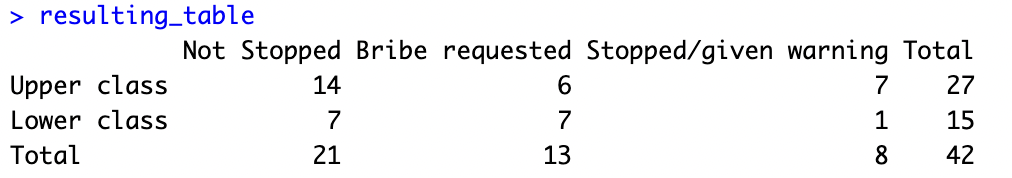
\includegraphics[width=1.1\textwidth]{1.1.png}
	  \end{figure}
	  
	  	Next, I need to calculate the expected frequency, as shown in Figure 2\\
	  	\begin{figure}[h!]
	  	\caption{\footnotesize{Expected Frequency table}}
	  	\vspace{.5cm}
	  	\centering
	  	\label{fig:1.2 Expected Frequency table}
	  	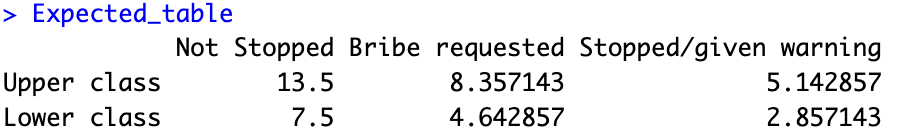
\includegraphics[width=1.1\textwidth]{1.2.png}
	  \end{figure}
	  
	  
	  Finally, according to the X-squared statistical calculation formula, I get:\\
	  	\begin{figure}[h!]
	  	\caption{\footnotesize{X-squared statistical calculation}}
	  	\vspace{.5cm}
	  	\centering
	  	\label{fig:1.3 X-squared statistical calculation}
	  	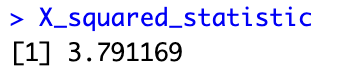
\includegraphics[width=0.5\textwidth]{1.3.png}
	  \end{figure}		
	\item [(b)]
	Now calculate the p-value from the test statistic you just created (in \texttt{R}).\footnote{Remember frequency should be $>$ 5 for all cells, but let's calculate the p-value here anyway.}  What do you conclude if $\alpha = 0.1$?\\
	\newpage
	\lstinputlisting[language=R, firstline=38, lastline=44]{PS02_answersZYZ.R}
	After calculation, the p value is 0.1502305\\
	\begin{figure}[h!]
	\caption{\footnotesize{p value}}
	\vspace{.5cm}
	\centering
	\label{fig:1.4 p_value}
	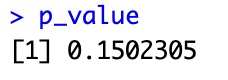
\includegraphics[width=0.5\textwidth]{1.4.png}
	\end{figure}

	If a is 0.1, then the confidence interval is 90, and the p-value is greater than 0.1, so the null hypothesis cannot be rejected. Therefore, there is no significant correlation between the driver’s class status and whether he is asked for a bribe.\\

	\item [(c)] Calculate the standardized residuals for each cell and put them in the table below.
	\vspace{1cm}
	
	\begin{table}[h]
		\centering
		\begin{tabular}{l | c c c }
			& Not Stopped & Bribe requested & Stopped/given warning \\
			\\[-1.8ex] 
			\hline \\[-1.8ex]
			Upper class  & 0.3220306 & -1.641957 & 1.523026 \\ 
			\\
			Lower class & -0.3220306 & 1.641957 & -1.523026 \\
			
			
		\end{tabular}
	\end{table}
	\lstinputlisting[language=R, firstline=45, lastline=66]{PS02_answersZYZ.R}	
	\begin{figure}[h!]
	\caption{\footnotesize{standardized residuals}}
	\vspace{.5cm}
	\centering
	\label{fig:1.6 standardized residuals}
	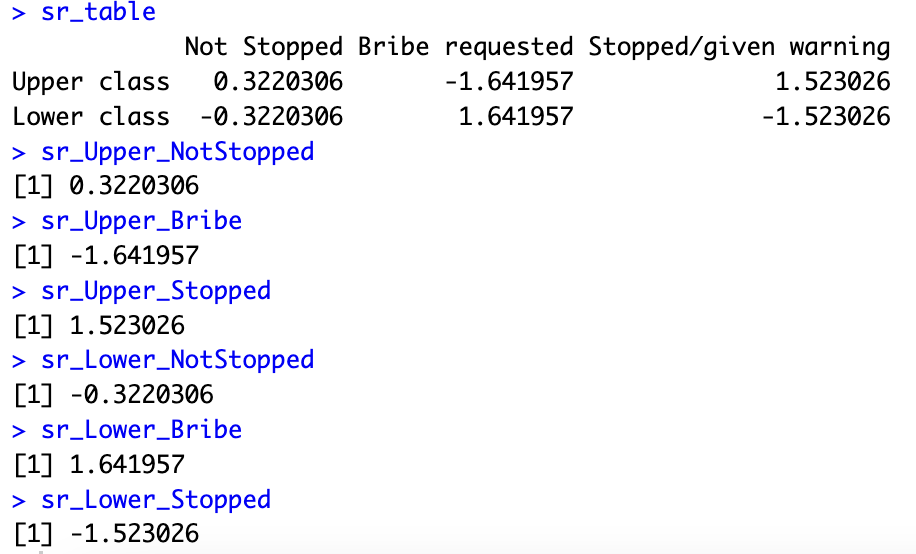
\includegraphics[width=1.1\textwidth]{1.5.png}
	\end{figure}
	\vspace{7cm}
	\item [(d)] How might the standardized residuals help you interpret the results? 
	\vspace{.5cm}
	 
	Upper Class\\
	(1)The value of the standardized residual for the upper class who has not been stopped is positive and relatively small (0.3220306), less than 1 and close to 0, indicating that this observation is slightly higher than the predicted value of the model, but the degree of deviation is not large.\\
	(2)The standardized residual value for the upper class who has been asked for a bribe is negative and relatively large (-1.641957), with an absolute value greater than 1 and less than 2, indicating that this observation is significantly lower than the predicted value of the model, and the degree of deviation is large, but it is still within a reasonable range.\\
	(3)The value of the upper class who has been stopped or warned is positive and relatively large (1.523026), greater than 1 but less than 2, indicating that this observation is significantly higher than the predicted value of the model, although the degree of deviation is large, but it is still within a reasonable range.\\
	Lower Class\\
	(1)The value of the standardized residual for the lower class who has not been stopped is negative and relatively small (-0.3220306), with an absolute value less than 1 and close to 0, indicating that this observation is slightly lower than the predicted value of the model, but the degree of deviation is not large.\\
	(2)The standardized residual value of the lower class being asked for bribes is positive and relatively large (1.641957), greater than 1 and less than 2, indicating that this observation is significantly higher than the model's predicted value, and the degree of deviation is large, but it is still within a reasonable range.\\
	(3)The standardized residual value of the lower class being stopped or warned is negative and relatively large (-1.523026), and the absolute value is greater than 1 but less than 2, indicating that this observation is significantly lower than the model's predicted value. Although the degree of deviation is large, it is still within a reasonable range.\\
	
	Conclusion\\
	The standardized residual values of the upper and lower classes being treated differently are all between [-2, 2], all within the normal range, and there are no abnormal values.The results passed the standardized residual test, and the hypothesis test model met the requirements.\\
\end{enumerate}
\newpage

\section*{Question 2: Economics}
Chattopadhyay and Duflo were interested in whether women promote different policies than men.\footnote{Chattopadhyay and Duflo. (2004). ``Women as Policy Makers: Evidence from a Randomized Policy Experiment in India. \textit{Econometrica}. 72 (5), 1409-1443.} Answering this question with observational data is pretty difficult due to potential confounding problems (e.g. the districts that choose female politicians are likely to systematically differ in other aspects too). Hence, they exploit a randomized policy experiment in India, where since the mid-1990s, $\frac{1}{3}$ of village council heads have been randomly reserved for women. A subset of the data from West Bengal can be found at the following link: \url{https://raw.githubusercontent.com/kosukeimai/qss/master/PREDICTION/women.csv}\\

\noindent Each observation in the data set represents a village and there are two villages associated with one GP (i.e. a level of government is called "GP"). Figure~\ref{fig:women_desc} below shows the names and descriptions of the variables in the dataset. The authors hypothesize that female politicians are more likely to support policies female voters want. Researchers found that more women complain about the quality of drinking water than men. You need to estimate the effect of the reservation policy on the number of new or repaired drinking water facilities in the villages.
\vspace{.5cm}
\begin{figure}[h!]
	\caption{\footnotesize{Names and description of variables from Chattopadhyay and Duflo (2004).}}
	\vspace{.5cm}
	\centering
	\label{fig:women_desc}
	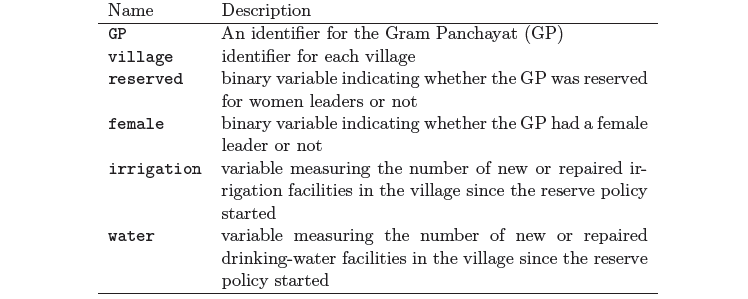
\includegraphics[width=1.1\textwidth]{women_desc.png}
\end{figure}		

\newpage
\begin{enumerate}
	\item [(a)] State a null and alternative (two-tailed) hypothesis. 
	
	Null Hypothesis: The reservation policy for women as village government leaders has no effect on the number of new or repaired drinking water facilities in the villages.\\
	
	Alternative Hypothesis: The reservation policy for women as village government leaders has positive/negative effect on the number of new or repaired drinking water facilities in the villages.\\
	\item [(b)] Run a bivariate regression to test this hypothesis in \texttt{R} (include your code!).
	\lstinputlisting[language=R, firstline=71, lastline=83]{PS02_answersZYZ.R}
	By observing the data and combining it with the variable explanation table, we can see that the values of the "women" variable and the "reserved" variable are the same. Therefore, I decided to use the "reserved" variable as the independent variable and "irrigation" and "water" as the dependent variables to explore their regression relationship.\\
	\vspace{8cm}
\begin{figure}[h!]
	\caption{\footnotesize{The binary regression bewteen irrigation and reserved}}
	\vspace{.5cm}
	\centering
	\label{fig:2.1 The binary regression bewteen irrigation and reserved}
	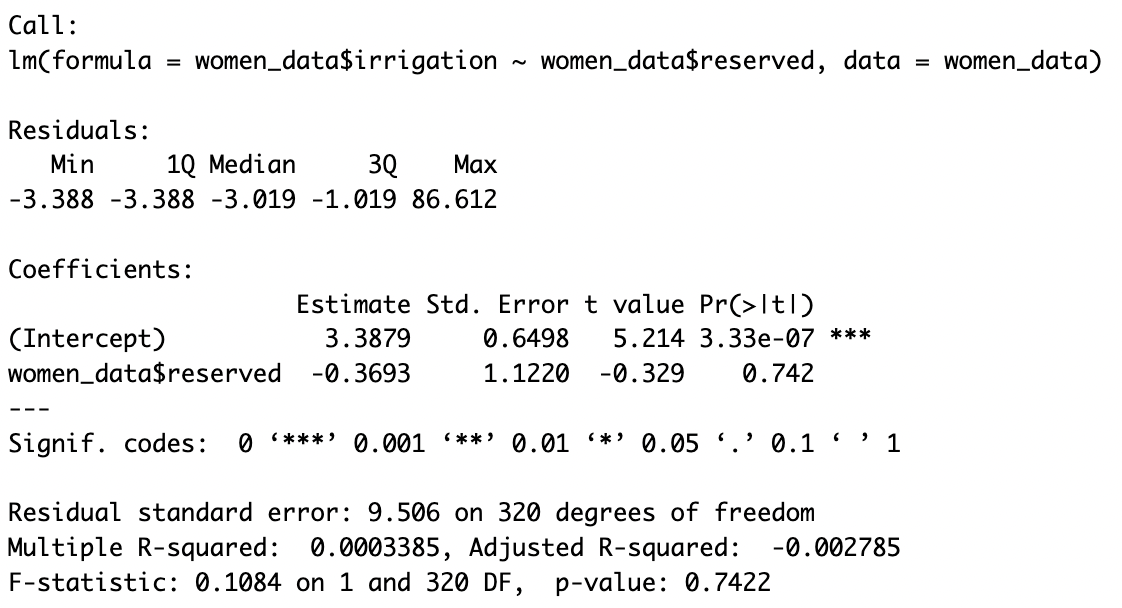
\includegraphics[width=1.1\textwidth]{2.1.png}
\end{figure}
	
	From the above figure, we can see that the p-value of the regression analysis of "irrigation" and "reserved" is 0.7422, which is much larger than 0.1, and the null hypothesis cannot be rejected. Therefore, there is no significant correlation between the implementation of the reservation policy and the number of irrigation facilities.\\
	
	
	Next, I will calculate the regression relationship between the variables water and reserved.\\
	\vspace{10cm}
\begin{figure}[h!]
	\caption{\footnotesize{The binary regression bewteen water and reserved}}
	\vspace{.5cm}
	\centering
	\label{fig:2.2 The binary regression bewteen water and reserved}
	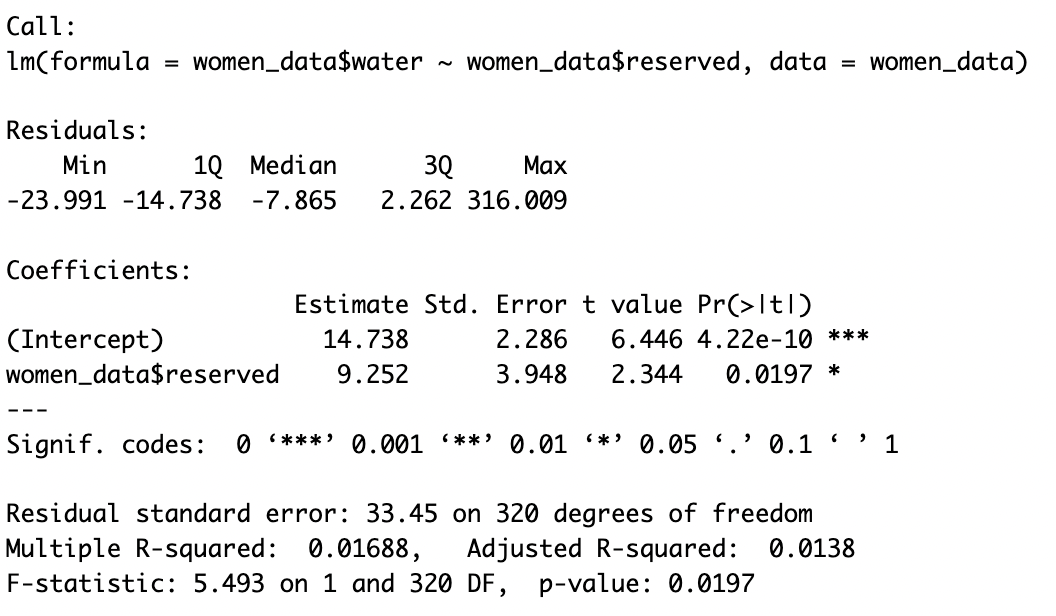
\includegraphics[width=1.1\textwidth]{2.2.png}
\end{figure}

	From the above figure, we can see that the p-value of the regression analysis of "water" and "reserved" is 0.0197, which is less than 0.05, and the null hypothesis is rejected. Therefore, there is a significant correlation between the implementation of the reservation policy and the number of drinking water facilities.\\
	\item [(c)] Interpret the coefficient estimate for reservation policy. \\
	
	The coefficient estimate of the regression model of water and reserved is 9.252, which is a positive number and shows a positive correlation. This usually means that if the independent variable reserved increases by one unit, the dependent variable water may increase by 9.252 units. Under this premise, it is possible that for every leadership position reserved for a woman, 9.252 drinking water facilities will be added. \\
	Assuming that the variables are linear and considering that the intercept is 14.738, we can get the relationship between reserved and water:\\ Y(water)=9.252*X(reserved)+14.738\\
\end{enumerate}

\end{document}
